\documentclass{beamer}

\usepackage[utf8x]{inputenc}
\usepackage[spanish]{babel} %Para configuración de idioma
\usepackage{amssymb}
\usetheme{OVA}

\setbeamertemplate{background canvas}{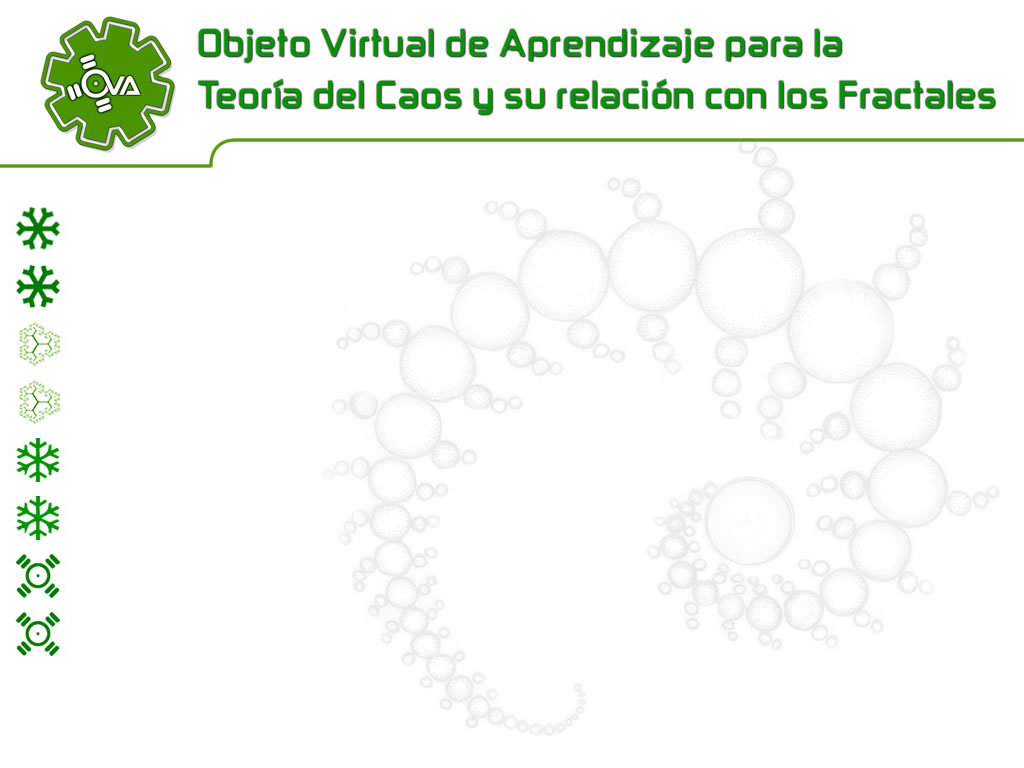
\includegraphics [width=\paperwidth,height=\paperheight]{fondo.jpg}}
\definecolor{verde}{RGB}{36,110,33}
\setbeamercolor{frametitle}{fg=verde}

\setbeamercolor{frametitle}{series=\bfseries}
\usepackage{hyperref}
%permite usar las transparencias de los los item. Se quita con \setbeamercovered{invisible}
\setbeamercovered{transparent}

%  \title{}
\author{Andrés Ricardo Torres Martínez  \\ Director \\ \texttt{Ing. Angel García Baños, Ph.D.}}
\institute{Escuela de Ingeniería de Sistemas y Computación\\ Universidad del Valle}
\date{15 de Febrero de 2011}
\begin{document}

%Buenos dias! 

\begin{frame}
\titlepage
\end{frame}

\begin{frame}
\frametitle{Introducción}
  \begin{itemize}
   \item Pedagogía + Informática =  Objeto virtual de aprendizaje.
   \item Computación evolutiva y Vida artificial: Algoritmos genéticos, complejidad, \textbf{teoría del caos} , auto-duplicación, teoría de juegos.   
   \item Metodología del docente $\blacktriangleright$ Auto aprendizaje.
  \end{itemize}
\end{frame}

\begin{frame}
\frametitle{Justificación}
El proyecto se origina dada la necesidad de mejorar el aprendizaje de la teoría del caos que se aborda de una manera superficial en la clase de computación evolutiva y mediante él se crea una aplicación web que permita a:

\begin{itemize}
\item La universidad:
  \begin{itemize}    
  \item Lograr optimizar el uso de sus recursos informáticos, haciendo un uso mayor y más eficaz de ellos.
  \item Aprovechar las nuevas tecnologías de información y comunicación con el propósito de actualizar sus procesos educativos.    
  \end{itemize}
\end{itemize}
\end{frame}

\begin{frame}
\frametitle{Justificación}

\begin{itemize}
 \item Los docentes:
  \begin{itemize}    
    \item Disponer de una nueva herramienta edumática que les permite aplicar y mejorar sus estrategias didácticas.
    \item Brindar nuevas posibilidades para la enseñanza.
    \item Agregar experiencia en el recorrido de la búsqueda del equilibrio en la educación virtual.
  \end{itemize}
  \item Los estudiantes:  
  \begin{itemize}    
    \item Un proceso de aprendizaje más lúdico e interactivo relacionado con conceptos de la teoría del caos.
    \item Apoyar su aprendizaje de acuerdo a su propio ritmo, permitiéndoles una mejor administración de su tiempo.
    \item Favorecer su desarrollo autónomo y a la vez la interacción colectiva.  
    \item Un sistema de autoevaluación mediante sencillos test para crear un ánimo de educación autodidacta.
  \end{itemize}
\end{itemize}

\end{frame}
\begin{frame}
\frametitle{Objetivo general}
Desarrollar una herramienta de aprendizaje interactiva para la enseñanza de la teoría del caos y su relación con los fractales aplicando conceptos de aplicaciones web. 
\end{frame}

\begin{frame}[label=OBJETIVOS]
  \frametitle{Objetivos específicos}
    \begin{itemize}
      \item <1>Diseñar e implementar un sistema web para el manejo de contenidos, o utilizar uno existente. \hyperlink{DRUPAL}{\beamergotobutton{Ver}}
      \item <2>Diseñar e implementar una aplicación con tecnologías web utilizando el manejador de contenidos. \hyperlink{EVA}{\beamergotobutton{Ver}}
      \item <3>Diseñar e implementar un visualizador de fractales de forma interactiva para su fácil aprendizaje.\hyperlink{FRACTAL}{\beamergotobutton{Ver}}
      \item <4>Diseñar el temario que se va a desarrollar como contenido de la aplicación centrada en la teoría del caos y su relación con los fractales. \hyperlink{CAOS}{\beamergotobutton{Ver}}
      \item <5>Diseñar pruebas de software y validarlas con alumnos de la asignatura computación evolutiva o interesados. \hyperlink{PRUEBA}{\beamergotobutton{Ver}}
    \end{itemize}
  \hypertarget<1>{OODRUPAL}{}
  \hypertarget<2>{OOEVA}{}
  \hypertarget<3>{OOFRACTAL}{}
  \hypertarget<4>{OOCAOS}{}
  \hypertarget<5>{OOPRUEBA}{}
\end{frame}

\begin{frame} [label=DRUPAL]
  \frametitle{Solución Propuesta}  
  \begin{itemize} 
  \item <1> El objeto virtual de aprendizaje es una aplicación web que permite gestionar fácilmente el contenido y permite adicionar funcionalidades: 
    \begin{itemize}
      \item Estructura de evaluación
      \item Estructura didáctica
      \item Estructura teórica
    \end{itemize}
  \item <2> Manejador de contenidos, Drupal :
    \begin{itemize}
      \item Contenido modular y configurable
      \item Roles, usuarios y seguridad
      \item Edición WYSIWYG (What Yor See Is What Your Get)
      \item Internacionalización
    \end{itemize}
  \item <2> \underline{\href{http://127.0.0.1/?q=es/node/3}{IR A Aplicación}} \hyperlink{OODRUPAL}{\beamergotobutton{Ver Objetivos}}
  \end{itemize}

\end{frame}

\begin{frame} [label=EVA]
  \frametitle{Drupal}
  
  \begin{columns}
    \begin{column}[l]{4cm}
     \pgfdeclareimage[width=3cm]{drupallogo}{Imagenes/drupal-logo.jpg}
      \pgfuseimage{drupallogo}<1>
      \pgfdeclareimage[width=4.5cm]{drupal}{Imagenes/drupal.png}
      \pgfuseimage{drupal}<2>
    \end{column}
    \begin{column}[l]{5cm}
      \begin{itemize}
        \item <1> Configuración del sistema.
	\item <2> Adaptación del gestor de contenidos, personalizando diversos módulos e implementando nuevas funcionalidades a través de la creación de módulos específicos.
      \end{itemize}

    \end{column}
  \end{columns}
\end{frame}

\begin{frame}
  \frametitle{Estructura de evaluación}
  \begin{itemize}
    \item <1>\underline{\href{http://127.0.0.1/?q=es/node/42}{Visualización} :} Se muestran las preguntas y las respuestas, ambas de forma aleatoria. Y se muestra solo la cantidad de respuestas visibles configuradas por pregunta.
    \item <2>\underline{\href{http://127.0.0.1/?q=es/node/1}{Configuración} :}
    \begin{itemize}
      \item Test: Un test por tema del temario principal.
      \item Pregunta: Las preguntas tienen peso variable, aunque por defecto, valen todas igual. Los pesos se normalizan para manejar varias escalas. 
      \item Respuesta: Las respuestas tienen peso variable, tiene mas peso la que mas correcta este, y un indicador si la respuesta es fija en la visualización.
    \end{itemize}
    \item <2> \hyperlink{OOEVA}{\beamergotobutton{Ver Objetivos}}
  \end{itemize}

\end{frame}


\begin{frame} [label=FRACTAL]
  \frametitle{Estructura didáctica}
  Dos mini aplicaciones, una para la navegación del fractal más famoso (conjunto de Mandelbrot) y otra para la construcción de fractales propios por medio de una interfaz.
\end{frame}

\begin{frame} 
 \frametitle{¿Que son los fractales?}
  Los fractales son representaciones gráficas de ciertos conjuntos de datos, los cuales generan repetición de patrones (parciales o totales) a lo largo de un dibujo.
  \begin{center}
    \pgfdeclareimage[width=6cm]{mandelbrot}{Imagenes/mandelbrot}
    \pgfuseimage{mandelbrot}
  \end{center}
\end{frame}


\begin{frame}
  \frametitle{Características de los fractales}   
  La palabra fractal viene del latín \textit{fractus} que significa fracturado. Este nombre se debe a que muchos poseen una estructura que al ser fragmentada se repite en diferentes escalas (auto similar).
  \begin{columns}
    \begin{column}[l]{5cm}
      \begin{itemize}
      \item <1> Conjunto de Mandelbrot sin aumento
      \item <2> Aumento de 4 veces
      \item <3> Aumento de 30 veces
      \item <4> Aumento de 350 veces
      \item <5> \underline{\href{http://127.0.0.1/index.php?q=node/66}{Conjunto de Mandelbrot}}
      \end{itemize}
    \end{column}
    \begin{column}[r]{5cm}
      \pgfdeclareimage[width=4.5cm]{Mandelbrot-similar1}{Imagenes/Mandelbrot-similar1.png}
      \pgfuseimage{Mandelbrot-similar1}<1>
      \pgfdeclareimage[width=4.5cm]{Mandelbrot-similar2}{Imagenes/Mandelbrot-similar2.png}
      \pgfuseimage{Mandelbrot-similar2}<2>
      \pgfdeclareimage[width=4.5cm]{Mandelbrot-similar3}{Imagenes/Mandelbrot-similar3.png}
      \pgfuseimage{Mandelbrot-similar3}<3>
      \pgfdeclareimage[width=4.5cm]{Mandelbrot-similar4}{Imagenes/Mandelbrot-similar4.png}
      \pgfuseimage{Mandelbrot-similar4}<4>
    \end{column}
  \end{columns}   
\end{frame}


\begin{frame}
\frametitle{Visualizador de fractales}
  \begin{itemize}
   \item HTML 5 
   \item Gramatica de sistemas de Lindemayer
   \begin{itemize}
    \item Simbolos :
      \begin{itemize}
      \item $[A-Z]$ Variables para seguir adelante y pintar.
      \item $+$ Gira en sentido de las aguajas del reloj.
      \item $-$ Gira en contra sentido de las aguajas del reloj.
      \end{itemize}
    \item Reglas de construcción
    \item Inicio
    \item Grados
   \end{itemize}  
  \end{itemize}
\end{frame}

\begin{frame}
\frametitle{Ejemplo Visualizador de fractales}
  \begin{itemize}
    \item Reglas de construcción : F $\rightarrow$ F-F++F-F
    \item Grados : 60 
    \item Inicio : F++F++F
    \item Iteraciones :
      \begin{itemize}
	\item Inicio : F++F++F
	\item Iteracion 1 : F-F++F-F ++ F-F++F-F ++ F-F++F-F
	\item Iteracion 2 : F-F++F-F-F-F++F-F++F-F++F-F-F-F++F-F ++ F-F++F-F-F-F++F-F++F-F++F-F-F-F++F-F ++ F-F++F-F-F-F++F-F++F-F++F-F-F-F++F-F
      \end{itemize}
  \item \underline{\href{http://127.0.0.1/index.php?q=node/67}{IR A Visualizador de fractales}}
  \item \hyperlink{OOFRACTAL}{\beamergotobutton{Ver Objetivos}}
  \end{itemize}  
\end{frame}

\begin{frame} [label=CAOS]
  \frametitle{Estructura teórica}
Selección de términos básicos e importantes y creación de un esquema de contenidos.
    El OVA cuenta con un contenido desarrollado de manera específica.
\begin{itemize}
  \item Dominio de contenidos
  \item Procesual
  \item Aprendizaje por descubrimiento
  \item Cambio conceptual
\end{itemize}
\hyperlink{OOCAOS}{\beamergotobutton{Ver Objetivos}}
\end{frame}

\begin{frame} [label=PRUEBA]
  \frametitle{Pruebas Realizadas}
\begin{itemize}
  \item <1> Diseño y realización de encuesta acerca de la usabilidad, entendimiento , comprensión , facilidad de manejo y comprensión de la aplicación,
  \item <2> Se realizaron 20 encuestas entre estudiantes de varios semestres de ingeniería de sistemas, para obtener una variedad con respecto a quienes han cursado la asignatura computación evolutiva y quienes no, además, también fue realizada a estudiantes de otras carreras interesadas como matemáticas y otras ingenierías para valorar el producto no solo como un desarrollo de software sino también como una herramienta útil de aprendizaje para diverso público interesado.
\end{itemize}
  
\end{frame}

\begin{frame}
\frametitle{Conclusiones}
\begin{itemize}
  \item <1>Los OVA tienen diversas posibilidades de uso, desde ayudar a la motivación y concentración de los estudiantes, hasta ser el soporte de una clase completa.
  \item <2>La complejidad de la teoría del caos, los insuficientes conocimientos de matemáticas y la falta de formación previa son los principales obstáculos para el proceso de aprendizaje.
  \item <3>La creación de recursos digitales como los OVA hace que la labor del docente se redimensione.
  \item <4>Las evaluaciones en una plataforma virtual muchas veces se realizan de una forma general, pueden llegan a ser predecibles y aburridas para los estudiantes, por lo que crear algo de aleatoriedad puede ayudar a mejorar la autoevaluación.  
\end{itemize} 
\end{frame}
\end{document}
